\section{Stability}
\subsection{Method}
\begin{frame}{Principle}
\begin{itemize}
\item Stable direct integration scheme:
\begin{equation*}
\exists h_0 > 0 \hspace{0.5cm}\text{such as} \hspace{0.5cm} \forall h \in [0,h_0]
\end{equation*}  
a finite perturbation of the state vector at $t_n$ gives a non growing modification of the state vector at an ulterior time $t_{n+j}$.
\item Equation of motion at time $t_{n}$ and $t_{n+1}$:
\begin{equation}
\begin{cases}
    M  \Ddot{U}^n = -C \Dot{U}^n - K U^n +P_{int}^n \\
    M \Ddot{U}^{n+1} = -C \Dot{U}^{n+1} - K U^{n+1} +P_{int}^{n+1} 
\end{cases}
\end{equation}
\item And the recurrence relationships by Newmark method (it could be another method):
\begin{equation}
\begin{cases}
\dot{U}_{n+1} = \dot{U}_n + (1-\gamma)dt \ddot{U}_n + \gamma dt \ddot{U}_{n+1} \\
U_{n+1} = U_n +dt \dot{U}_n + dt^2 \left(\frac{1}{2}-\beta\right) \ddot{U}_n + dt^2 \beta \ddot{U}_{n+1}
\end{cases}
\end{equation}
\end{itemize}
\end{frame}

\begin{frame}{Principle (2)}
\begin{itemize}
\item Combining the two:
\begin{equation}
\resizebox{\columnwidth}{!}{

    M \dot{u}^{n+1} = M\Dot{u}^{n} + h(1-\gamma)\left[ -C \Dot{u}^n -
     K u^n +p_{int}^n   \right] + \gamma h \left[ -C \Dot{u}^{n+1} - K u^{n+1} +p_{int}^{n+1} \right] 

}
\end{equation}
\end{itemize}
\end{frame}

\begin{frame}{1D: four cases}
\begin{figure}[ht] 
  \label{ fig7} 
  \begin{minipage}[b]{0.5\linewidth}
    \centering
    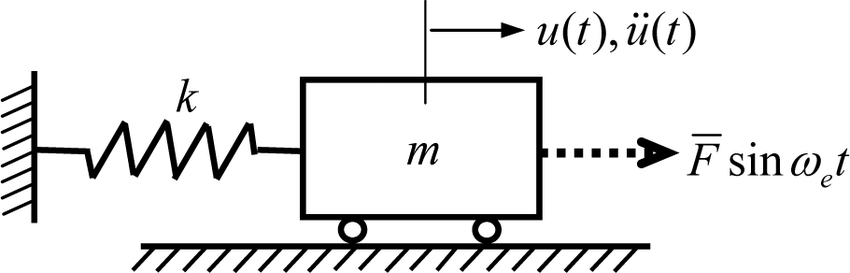
\includegraphics[width=.5\linewidth]{images/sdof-spring.png} \\
    Single degree of freedom spring
    \vspace{4ex}
  \end{minipage}%%
  \begin{minipage}[b]{0.5\linewidth}
    \centering
    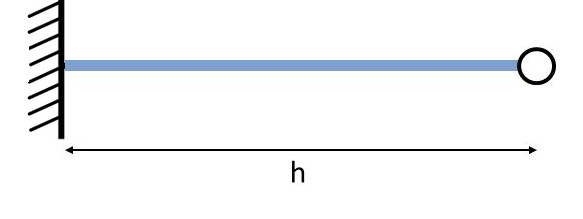
\includegraphics[width=.5\linewidth]{images/encastred.jpg} \\
    Fixed extremity 1D bar element
    \vspace{4ex}
  \end{minipage} 
  \begin{minipage}[b]{0.5\linewidth}
    \centering
    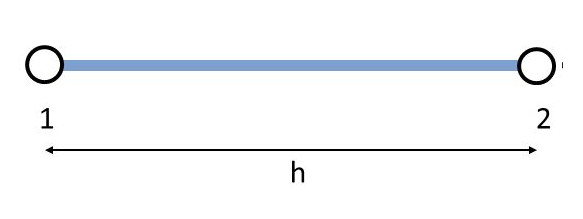
\includegraphics[width=.5\linewidth]{images/bar-element.jpg} \\
    1D bar element
    \vspace{4ex}
  \end{minipage}%% 
  \begin{minipage}[b]{0.5\linewidth}
    \centering
    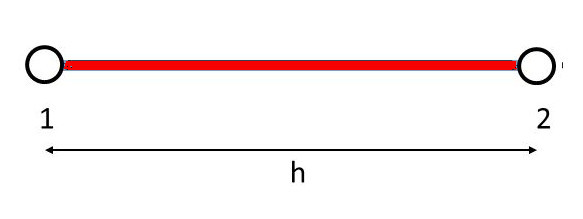
\includegraphics[width=.5\linewidth]{images/bar-element-pml.jpg} \\
    1D PML bar element
    \vspace{4ex}
  \end{minipage} 
\end{figure}
\end{frame}
